\Solution{1: Multi-armed Bandits}
\begin{enumerate}
    \item Created the environment using Gymnasium library. The environment is a 2-armed bernoulli bandit with some stochasticity. The environment characteristics are taken from a config file which specify the $\alpha$ and $\beta$ values. I tested out with different values of $\alpha$ and $\beta$ $[(0,0), (0,1), (1,0), (1,1), (0.5,0.5)]$ and the environment is working as expected. The agent recieves a reward only if it takes an action which takes it correctly in the direction of movement. That is if the the agent moves `left' and lands in state $1$ or moves `right' and lands in state $2$, only then it gets a positive reward. 
    
    \item I created a similar environment with 10-arms just like the above. But in this case the environment is not stochastic. The action and state-transitions are deterministic. The expected reward for each action $q_*(s, a)$ is sampled from a standard normal distribution ($\mathcal{N}(0, 1)$). The agent then receives a reward from a normal distribution with mean $q_*(s, a)$ and variance $1$. The agent has to then learn the optimal action to take in each state, by taking actions and observing the rewards.
    
    \item I created 6 types of bandit agents following different strategies to solve the bandit problem. The agents are:
    \begin{enumerate}
        \item Greedy Agent: This agent always takes the action with the highest estimated value. It does not explore the environment.
        \item Epsilon-Greedy Agent: This agent takes the action with the highest estimated value with probability $1-\epsilon$ and takes a random action with probability $\epsilon$.
        \item Decaying Epsilon-Greedy Agent: This agent is similar to the epsilon-greedy agent, but the value of $\epsilon$ decays ``linearly'' $\epsilon=max(0, \epsilon_0 - decay\_rate * episode)$ or ``exponentially'' $\epsilon=\epsilon_0e^{-decay\_rate*episode}$ with time. 
        \item Softmax Agent: This agent takes actions with probability proportional to the exponential of the estimated value of the action. The agent explores the environment by taking actions by choosing from the below distribution
        \begin{equation}
            \pi(a|s) = \frac{e^{Q(s,a)/\tau}}{\sum_{b}e^{Q(s,b)/\tau}}
        \end{equation}
        \item UCB Agent: This agent takes actions by choosing the action with the highest upper confidence bound. The upper confidence bound is calculated as $Q(s,a) + c\sqrt{\frac{\ln t}{N(s,a)}}$ where $c$ is a constant and $N(s,a)$ is the number of times the action $a$ has been taken in state $s$. The action is taken by taking the argmax of the upper confidence bound. 
    \end{enumerate}
    
    \item Created 50 different bandit problems for 2-armed Bernoulli Bandit with $\alpha$ and $\beta$ values chosen from uniform distribution $\mathcal{U}(0, 1)$. The agents were then tested on these bandit problems. The agents were tested for 1000 episodes and the average reward, average regret and optimal action percentage was calculated. The results are shown in the plots below (Figure \ref{fig:bernoulli_reward}, \ref{fig:bernoulli_regret}, \ref{fig:bernoulli_optimal_action}). 
    
    \item Created 50 different bandit problems for 10-armed Gaussain Bandit with $q_*(s, a)$ values chosen from standard normal distribution $\mathcal{N}(0, 1)$ and then the agent receives a reward from $\mathcal{N}(q_*(s, a), 1) \forall a \in A$. The agents were then tested on these bandit problems for 1000 episodes and the average reward, average regret and optimal action percentage was calculated. The results are shown in the plots below (Figure \ref{fig:gaussian_reward}, \ref{fig:gaussian_regret}, \ref{fig:gaussian_optimal_action}).
    
    \begin{figure}[h]
        \centering
        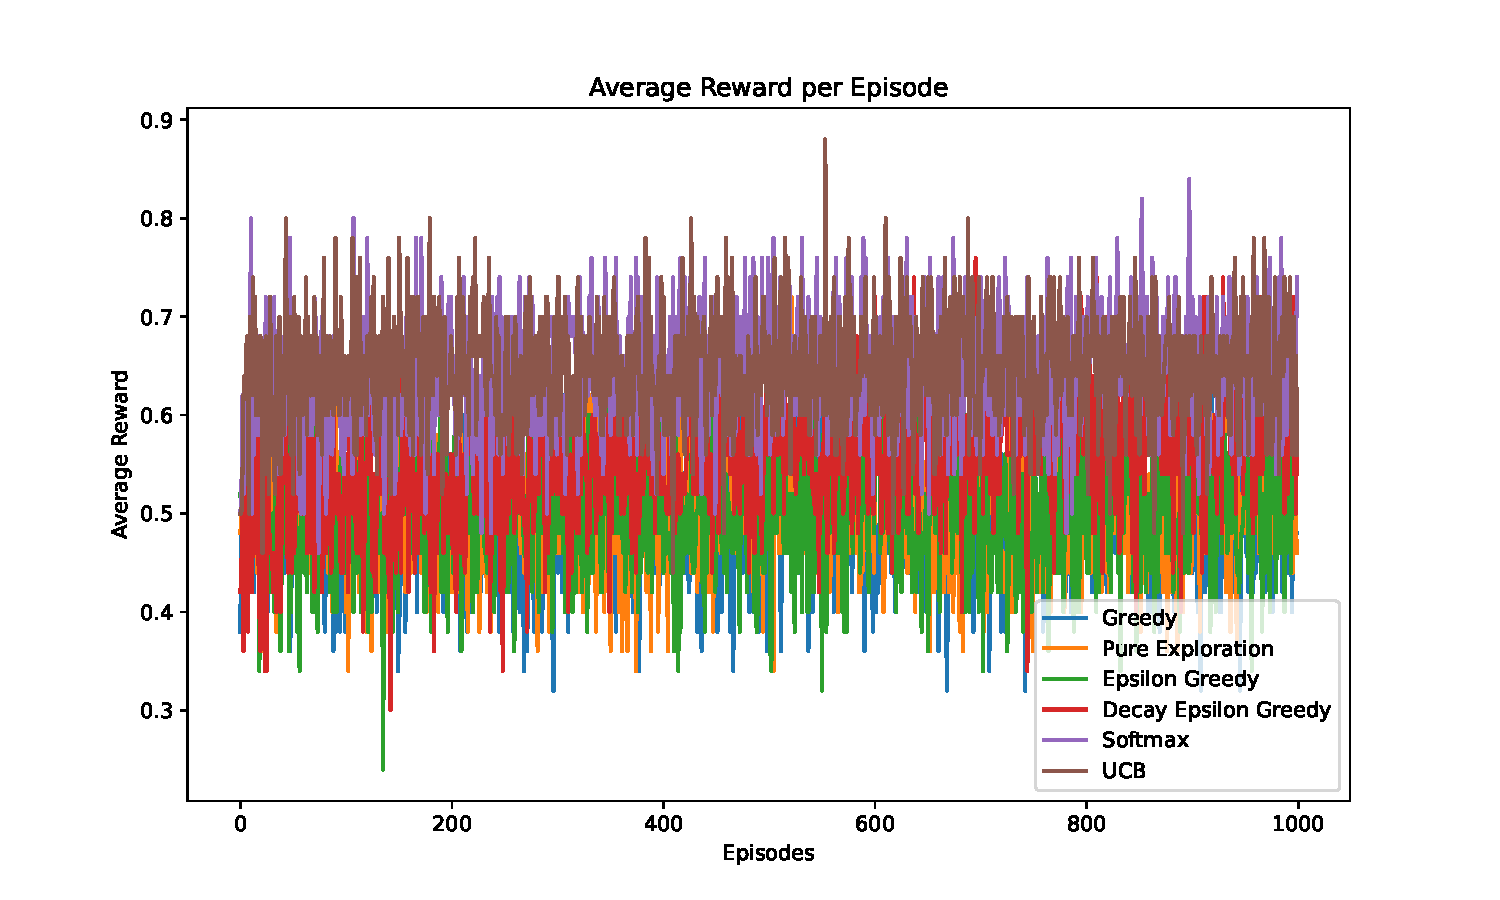
\includegraphics[width=0.8\textwidth]{images/mab/bernoulli_average_reward_per_episode.pdf}
        \caption{Average reward of 2-armed Bernoulli Bandit}
        \label{fig:bernoulli_reward}
    \end{figure}

    \begin{figure}[h]
        \centering
        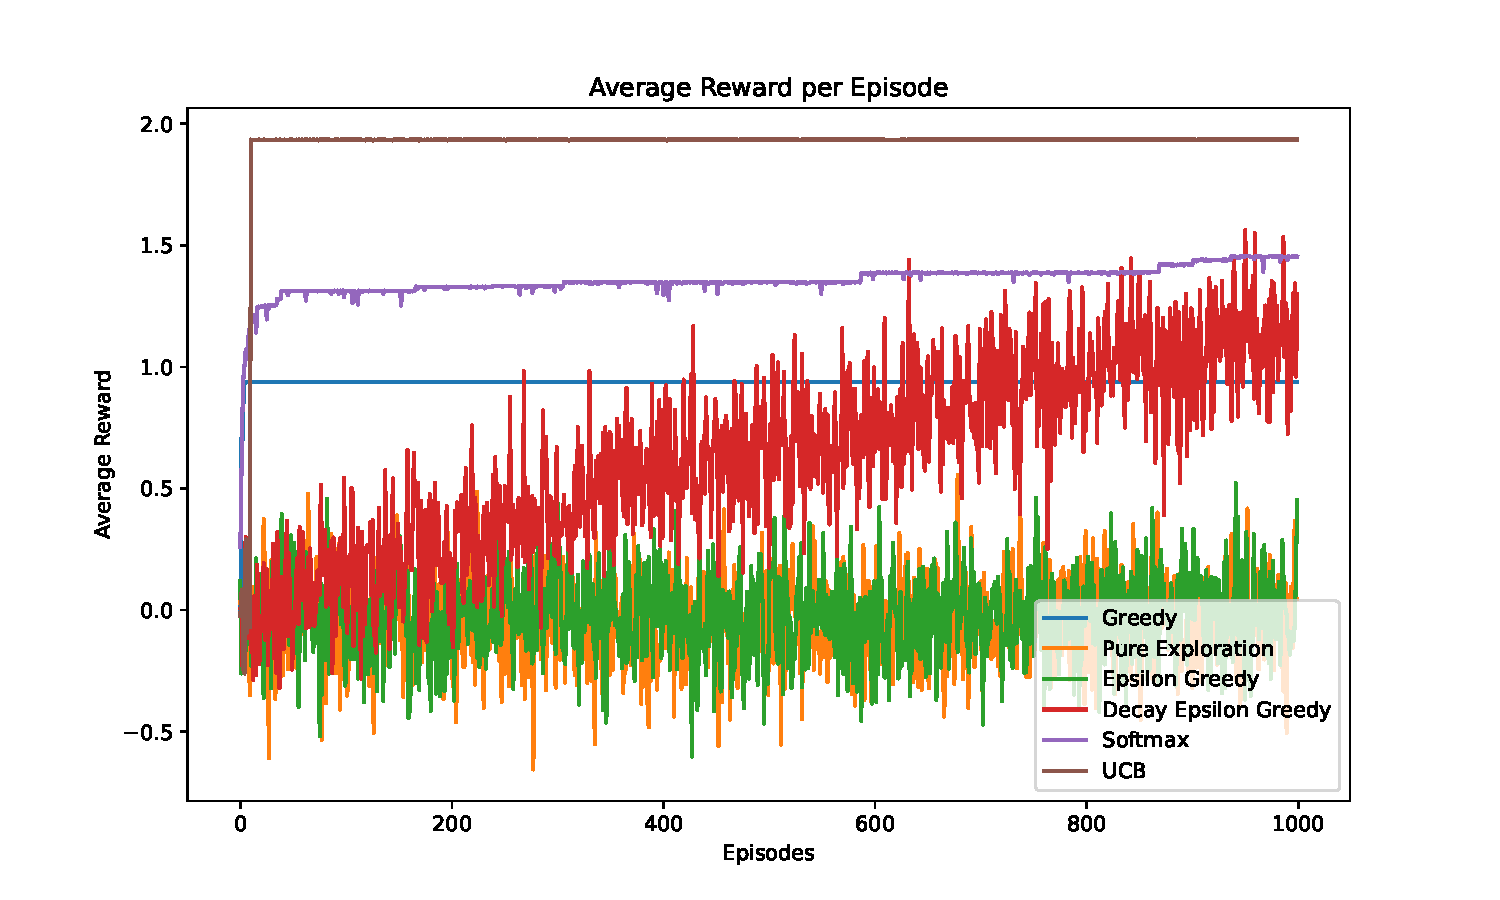
\includegraphics[width=0.8\textwidth]{images/mab/10_arm_gaussian_average_reward_per_episode.pdf}
        \caption{Average reward of 10-armed Gaussian Bandit}
        \label{fig:gaussian_reward}
    \end{figure}

    \item Created a plot of the average regret of the agents for the 2-armed Bernoulli Bandit. 
    \begin{figure}[h]
        \centering
        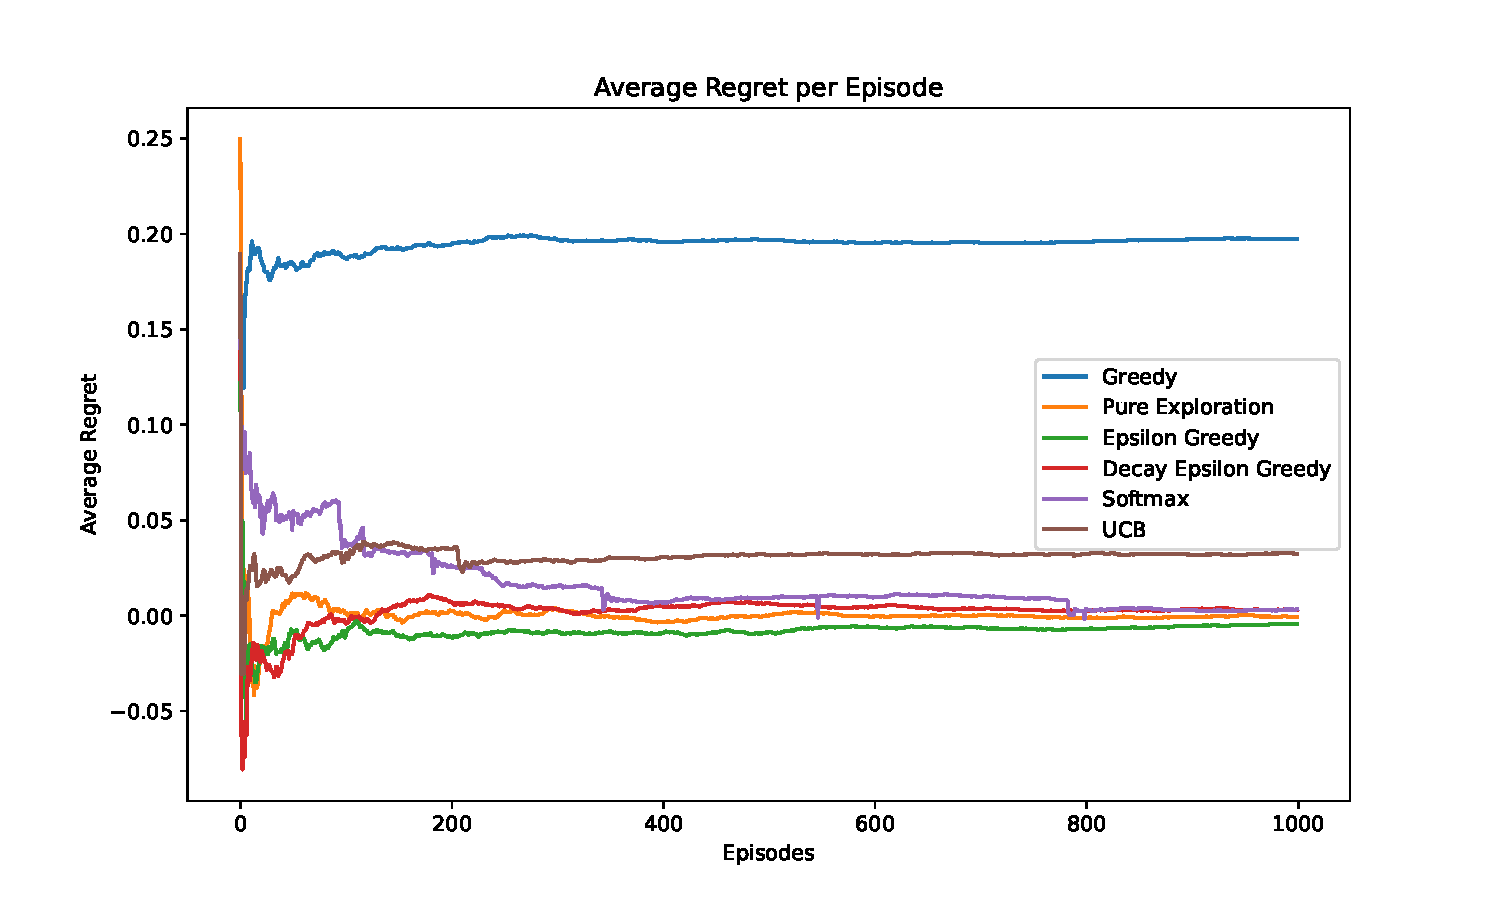
\includegraphics[width=0.8\textwidth]{images/mab/bernoulli_average_regret_per_episode.pdf}
        \caption{Average regret of 2-armed Bernoulli Bandit}
        \label{fig:bernoulli_regret}
    \end{figure}

    \item Created a plot of the average regret of the agents for the 10-armed Gaussian Bandit.
    \begin{figure}[h]
        \centering
        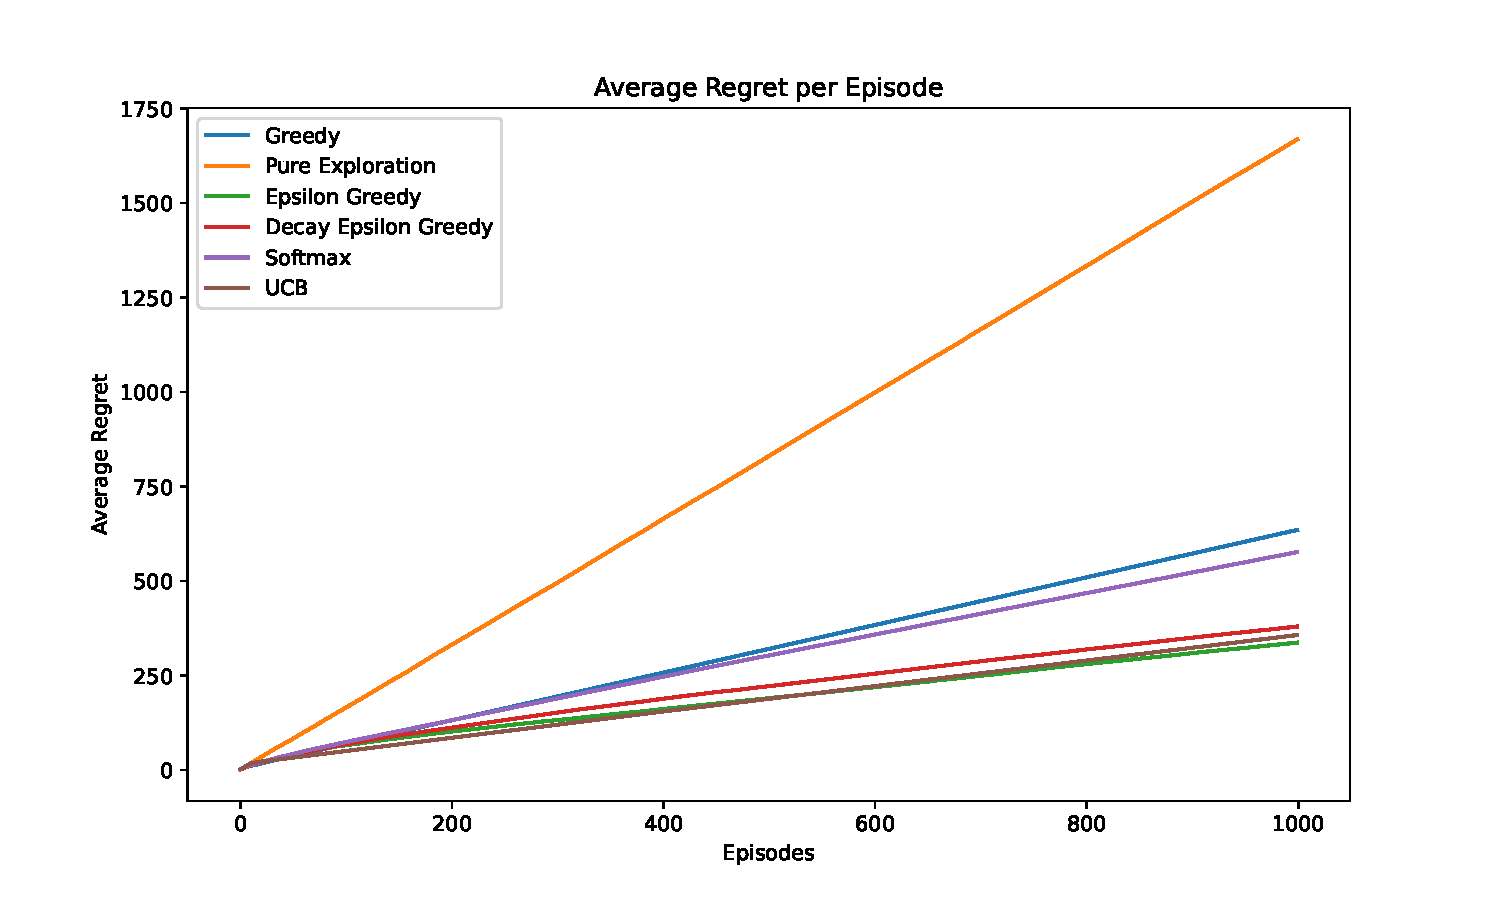
\includegraphics[width=0.8\textwidth]{images/mab/10_arm_gaussian_average_regret_per_episode.pdf}
        \caption{Average regret of 10-armed Gaussian Bandit}
        \label{fig:gaussian_regret}
    \end{figure}

    \item This is the same as question 4. 
    
    \item Plotting the optimal action percentage of each agent for the 2-armed Bernoulli Bandit.
    \begin{figure}[h]
        \centering
        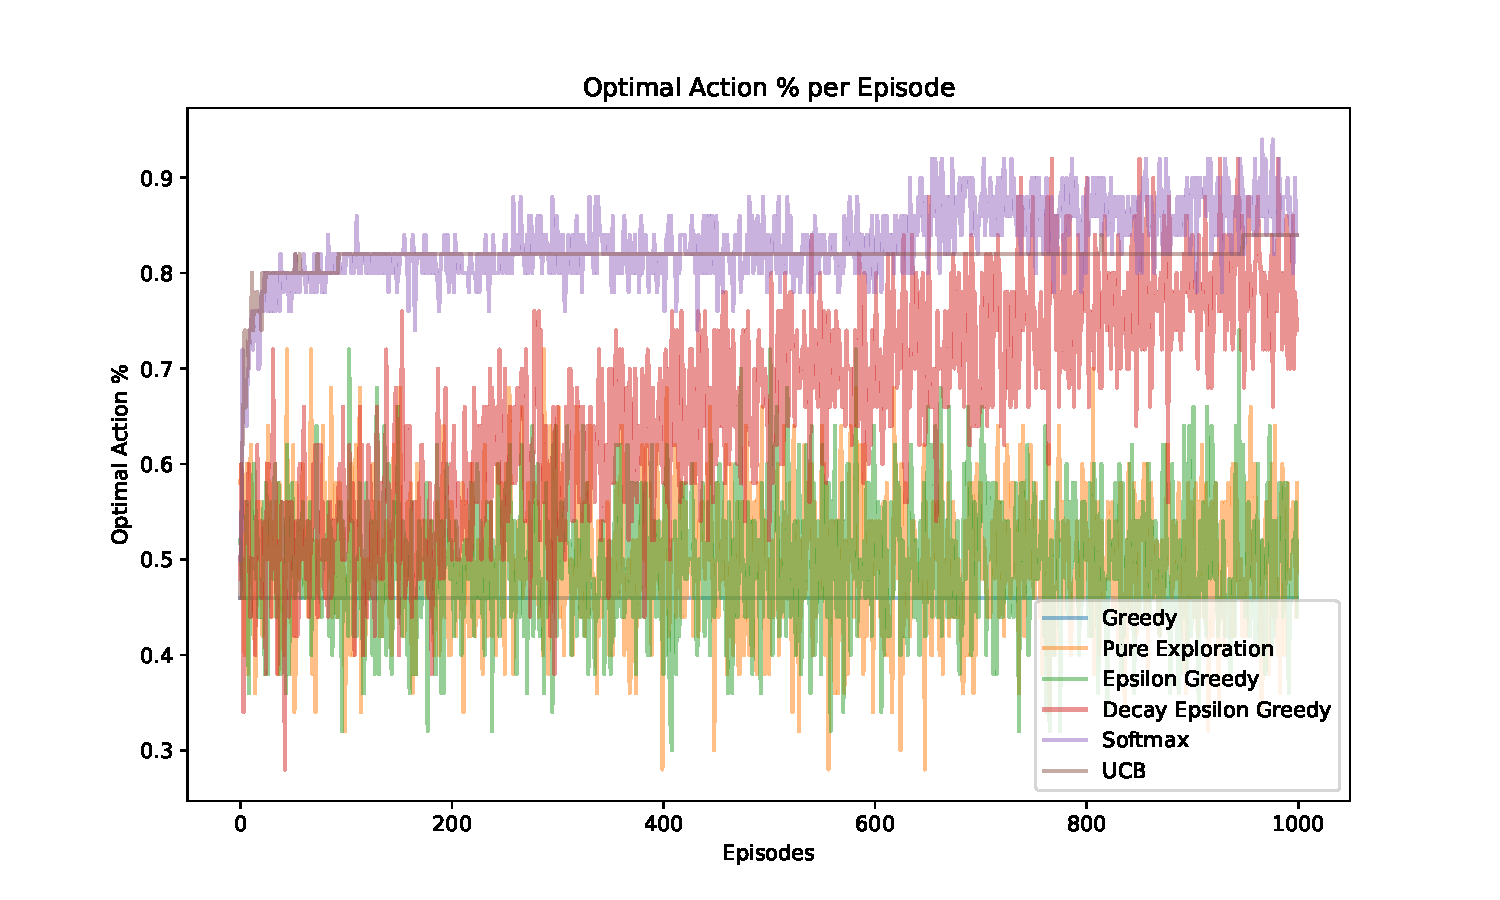
\includegraphics[width=0.8\textwidth]{images/mab/bernoulli_optimal_actions_percentage_per_episode.pdf}
        \caption{Optimal Action \% of 2-armed Bernoulli Bandit}
        \label{fig:bernoulli_optimal_action}
    \end{figure}

    \item Plotting the optimal action percentage of each agent for the 10-armed Gaussian Bandit.
    \begin{figure}[h]
        \centering
        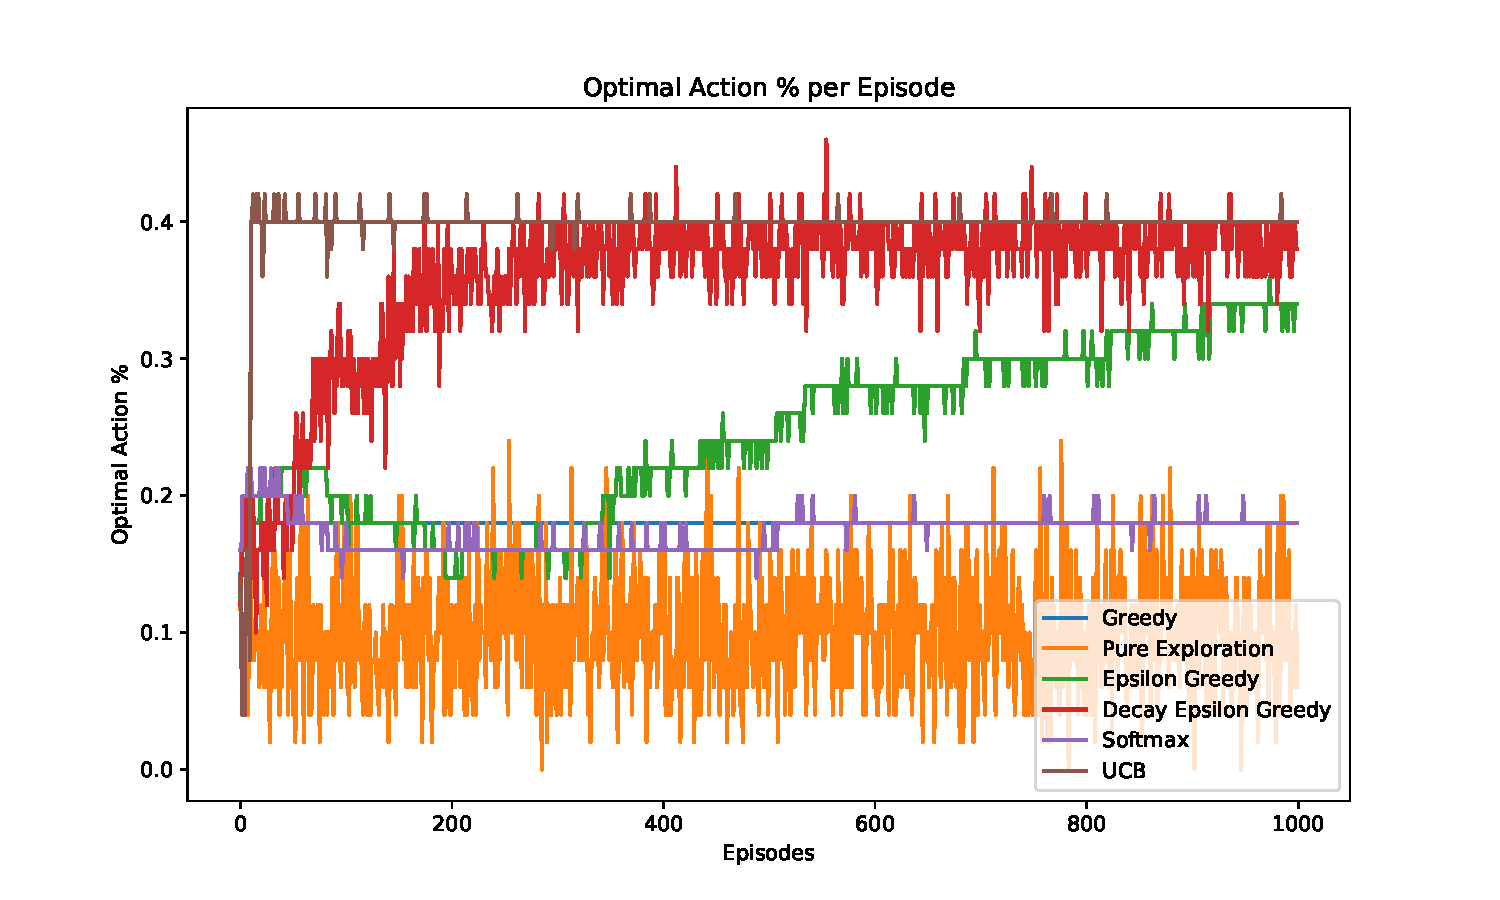
\includegraphics[width=0.8\textwidth]{images/mab/10_arm_gaussian_optimal_actions_percentage_per_episode.pdf}
        \caption{Optimal Action \% of 10-armed Gaussian Bandit}
        \label{fig:gaussian_optimal_action}
    \end{figure}

\end{enumerate}